\def\BibTeX{{\rm B\kern-.05em{\sc i\kern-.025em b}\kern-.08em
    T\kern-.1667em\lower.7ex\hbox{E}\kern-.125emX}}

\documentclass{article}
\usepackage[dvips]{graphicx}
%\usepackage{txfonts}
%\usepackage[T1]{fontenc}
\usepackage{array}
\usepackage{enumerate}
\usepackage{setspace}
\usepackage{fullpage}
\usepackage{url}
\usepackage[dcucite]{harvard}
\usepackage{amsmath}

%\usepackage[nofiglist,notablist]{endfloat}

\newcommand{\vk}[1]{\mbox{\boldmath $#1$}}

\title{Prices, Location Choices and Neighborhood Composition in a Dynamic Housing Market:
Towards a Unified Micro-level Model for Policy Analysis.
}


\author{Liming Wang \\ Department of Urban Design and Planning, \\
University of Washington \\ lmwang@u.washington.edu \and
Paul Waddell \\ Evans School of Public Affairs, \\
University of Washington \\ pwaddell@u.washington.edu}

\date{}

\begin{document}

\maketitle

\doublespacing
\begin{abstract}
  This paper develops two complementary models of the housing market as a preliminary effort
  to develop a unified model of the interactions among buyers and sellers in the market that
  we think will provide a robust basis for evaluating alternative policy interventions to deal
  with the adverse consequences of housing market dynamics such as displacement induced by
  gentrification of inner-city neighborhoods. The first model is a discrete choice model of
  household residential location choice.  The second is a random bidding model that predicts
  the household type of winning bidders and the winning transaction price for properties in an
  auction approach.  We estimate these models using data for the Puget Sound region containing
  Seattle, Washington, and develop a proposed approach to integrating them into a consistent
  micro-level model of the housing market.
\end{abstract}

\pagebreak

\section{Introduction}
\label{intro}
Between 1975 and 1995, real single-family home prices in
the United States increased by an average of .5 percent per
year, or 10 percent over the course of two decades. By
contrast, from 1995 to 2004, national real home prices rose by
3.6 percent per year, or nearly 40 percent in one
decade ~\cite{Shiller2006,Shiller2005}. With housing
costs representing the single largest expenditure item in
the average household budget, the rapid rise in prices -- even with the current
cooling in the housing market occurring in many parts of the country -- has a
substantial impact on most households.

The rapid rise in housing price clearly affects
of households differently depending on their circumstances. It makes
homeownership for first-time home owner more difficult, but
provides substantial capital gains for the group of
existing home owners. \citeasnoun{Quigley2004}
show that, by taking into account capital
gains, depreciation, property taxes and Federal taxes, the user
cost of housing for existing owners has not increased
significantly, but they agree that housing is becoming
less affordable for first-time owners and for renters, especially
low income renters. (See also, \cite{Quigley2005,Himmelberg2005}.) 

Another trend that bears on housing affordability for how income households is
the recent resurgence in interest among middle and upper income households in
central-city neighborhoods close to urban amenities.  Possible
causes for this return to the city shift include the growing levels of traffic
congestion associated with rising urban decentralization and a decline in
highway expansion in the past two decades. There is growing evidence that
gentrification of inner-city neighborhoods is occurring more frequently,
with attendant problems of displacement of low-income renters to
more remote suburban or exurban areas with lower levels of access to employment
opportunities and services, particularly via public transportation.

Analysis of intra-metropolitan housing market dynamics is needed in order to
assess the potential for mitigating the adverse consequences on low-income
households of these recent trends by alternative policy interventions.  Would
rental subsidies be more effective at mitigating these impacts, or would supply
subsidies, or improved transportation services, or other policies in combination?
In order to begin to approach this kind of policy evaluation, unfortunately, we
must first have a sufficiently robust understanding of the dynamics and a tractable
model to represent the potential impacts of alternative policy interventions.  In this
paper we draw on two existing approaches to addressing the underlying behavior in the
housing market that shape intra-metropolitan housing market dynamics, apply them and
address their capacity to represent these market dynamics.  We close with a preliminary
formulation of an approach to integrate these two approaches into a more robust
model for housing market analysis.

An alternative approach that we draw on but do not directly use is hedonic regression, which attempts to
decompose observed housing prices into implicit market valuation of a vector of
house characteristics $X$, including locational amenities ~\cite{Rosen1974a,Sheppard1999}.
Hedonic regression has become an extremely popular approach in the literature analyzing housing prices and the
implicit valuation of specific attributes of housing, ranging from
structural characteristics to environmental amenities.  This methodology
does not illuminate the underlying structure of demand or supply, however,
and is therefore not a sufficiently robust basis for our desired research on the dynamics
of housing markets from a more structural perspective, which we deem as essential in order to analyze
alternative policy interventions.  Hedonic regression
is essentially a reduced form representation of the market, assuming it is
in equilibrium, of the market valuation of housing attributes.  It is not
possible to derive directly from a hedonic regression information about the
underlying structure of demand functions of consumers by type, nor the
supply functions of housing providers.  Hence our interest in developing
a more structural representation of housing demand at the consumer level, and the
interaction of these demands among competing consumers to ration scarce supply among
competing consumers.

The first approach we draw on is the formulation of housing demand at the
individual household level via discrete choice models of location choice. This approach
was pioneered by \citeasnoun{mcfadden-1974} in his development of the Random Utility Maximization
theory and the discrete choice models that follow from them.  Numerous studies have
used and extended this approach, mostly by applying the common Multinomial Logit (MNL)
model structure to predict the probability that a household with a particular set of
characteristics will choose a particular housing unit or location from a set of available
alternatives.  The approach has been used widely in the literature on household location
choice (see for example, \cite{Quigley1976,Waddell2000}).  We apply this approach to the estimation of household location choice within
the Central Puget Sound region centered on Seattle, Washington, using locations specified
by small grid cells of 150 by 150 meters.

The second approach we use is based on the random bidding model developed by
Ellickson~\citeyear{ellickson1977b}.  This approach focuses on the problem
from the perspective of the seller, rather than the consumer, of housing.  It
develops an auction model that predicts the probability that a household of type
$t$ will be the highest bidder for a specified house or location.  In an extension by
Lerman and Kern~\citeyear{Lerman1983}, the random bidding model is adapted to predict
both the type of household of the winning bidder, as well as the value of the winning
bid -- that is to say, the transactions price of the property.  It is this extended
formulation that we use as the second approach in this paper.

Taken together, these two models offer complementary views of the housing market.  The first
reflects the housing consumer perspective, that is, the probability of selecting a particular
house or location from the available set of alternatives, given their characteristics and prices.
This perspective is valuable for formulating demand, but does not explicitly reflect the role
of competition among households in the market.  In other words, it does not address the rationing
problem of allocating scarce housing to competing consumers.  It also assumes that prices are
exogenous.  The second approach deals explicitly with the rationing problem using an auction framework,
and predicts prices endogenously.  This approach, however, does not address the composition of
consumers at each auction, which is directly addressed by the location choice framework.  We propose
an integration of these two approaches into a unified model of the housing market, and develop
a preliminary approach to this integration.

In the following sections, we first develop a household location choice model for the Puget Sound region,
and present and discuss estimation results from this model.  Then we develop and estimate a random bidding
model of the housing market for the Puget Sound region, and present and discuss estimation results.  We then
close with discussion of plans for the integration of these models, including a preliminary specification.

\section{Model Development}
\subsection{Household Location Choice Model}

In this section we develop a discrete choice model of household location choice,
drawing on the Random Utility Maximization (RUM) framework pioneered by Daniel
McFadden, who won a Nobel Prize in Economics for this and related work
\cite{mcfadden-1974,mcfadden-1981}. For each household, we assume that
each alternative $i$ has associated with it a utility $U_i$ that
can be separated into a systematic part and a random part:
\begin{equation}
    U_i = u_i + \epsilon_i,
    \label{eq:utility}
\end{equation}
where $u_i = \vk{\beta}\cdot\vk{x}_i$ is a linear-in-parameters
function, $\vk{\beta}$ is a vector of $k$ estimable coefficients,
$\vk{x}_i$ is a vector of observed, exogenous, independent
alternative-specific variables that may be interacted with the
characteristics of the agent making the choice, and $\epsilon_i$
is an unobserved random term. Assuming the unobserved term in
(\ref{eq:utility}) to be distributed with a Gumbel distribution
leads to the familiar multinomial logit model
\cite{mcfadden-1974,mcfadden-1981}:
\begin{equation}
    P_i = \frac{\mathrm{e}^{u_i}}{\sum_j \mathrm{e}^{u_j}},
    \label{eq:mnl}
\end{equation}
where $j$ is an index over all possible alternatives. The
estimable coefficients of (\ref{eq:mnl}), $\vk{\beta}$, are
estimated with the method of maximum likelihood (see for example
\cite{Greene-2002}).

We define alternatives as locations measured by grid cells of 150 by 150 meters.  We
use data from a 1999 Puget Sound Transportation Survey to obtain the observed locations
of households that had moved into their residence within the past five years.  To form a
choice set from the almost 800,000 alternative grid cells, we sample nonchosen alternatives
randomly to create a tractable size of alternative sets with which to estimate the model.
Note that this sampling of alternative approach depends on a property of the MNL model known
as the Independence of Irrelevant Alternatives (IIA) property, and has been shown to produce
consistent estimates of the model parameters \cite{mcfadden-1978}.

We include in the model specification first the interaction of household income and housing cost,
reflecting the housing cost burden.  We expect of course that households prefer lower-priced
alternatives when all else is equal.  It is this aspect of the model that would be directly useful
in examining the shifts in consumer location preferences as the relative prices of housing in
suburban and inner-city neighborhoods change over time.

The model specification also includes the classical urban economic trade-off between
transportation and land cost. This has been generalized to account
for access to employment opportunities distributed throughout the metropolitan
area, using travel times by auto and transit modes that are derived from the
Puget Sound Regional Council regional travel model system.  Taste for land is included by
measures of housing density at each location and within walking distance of that location.  We also
test for interactions between household characteristics, such as the presence of children, and this
taste for land, with an expectation that families will have a stronger preference for low-density
locations and neighborhoods than non-family households.

We include in the specification the interaction of household income with housing quality,
measured by the building value of the house; and with the income composition of the neighborhood.  We
expect households of higher income not only to prefer locations with higher quality housing, but also
to prefer neighborhoods with a higher proportion of higher income households. We also include the
interaction of the ethicity of the household choosing a location and the ethnic composition of the
neighborhood, to reflect segregation tendencies within the housing marker.

These independent variables can be organized into the three
categories of housing characteristics, regional accessibility, and
urban-design scale effects as shown in Table~\ref{table-variables}.

\begin{table}
\begin{center}
\caption{Independent Variables} \label{table-variables}
% Table generated by Excel2LaTeX from sheet 'Sheet2'
\begin{tabular}{lp{4in}}

\multicolumn{ 2}{l}{{\bf Housing Characteristics}} \\
\hline
           & housing age (year built) \\

           & number of bedrooms \\

           & number of bathrooms \\

           & structure type (single family home, duplex, etc) \\

           & building square feet \\

           & lot square feet / acres \\

           & residential units in parcels \\

           &    stories \\

           & imrpovement value \\

           &            \\

\multicolumn{ 2}{l}{{\bf Regional Acessibility}} \\
\hline
           & travel time to CBD \\

           & travel time to airport \\

           & number of jobs within 30 mins of driving \\

           & number of jobs within 30 mins of transit ride and walk \\

           & generalized cost weighted access to employment \\

           & travel time weighted access to employment \\

           &            \\

\multicolumn{ 2}{l}{{\bf Urban Design-scale Characteristics, Neighorhood Land Use}} \\
\hline
           & residential units within walking distance (600 meters) \\

           & housing density within walking distance \\

           & population density within walking distance \\

           & retail employment within walking distance \\

           & service employment within walking distance \\

           & total employment within walking distance \\

           & percent high income households within walking distance \\

           & percent low income households within walking distance \\

           & percent minority households within walking distance \\

           & percent residential land within walking distance \\

           & percent commercial land within walking distance \\

           & percent industrial land within walking distance \\

           & percent open space within walking distance \\
\hline
           &            \\

\end{tabular}  


\end{center}
\end{table}

Estimation results of this model are reported in Section \ref{results}.


\subsection{Random Bidding Model}

Bid-rent theory, on which much of urban economics is based, directly models the
competition among households for residential location as a
bidding process. In the housing market, households derive
utility from housing and consumption of other goods given
budget constraints, as well as commute cost and time
constraints. In equilibrium, every household achieves its
maximum utility subject to the budget constraints, while
housing price in every location adjusts to clear the market,
with price at the city boundary equal to
argriculture rent~\cite{alonso1965}. Bid rent theory has provided
a foundation for an extensive literature surrounding the monocentric
model and various extensions of it, but it does not provide an empirical
basis for estimating the structure of housing demand and prices that is
amenable to empirical analysis of real housing markets with all their
attendant complexity.

Bid rent theory was brought together with discrete choice theory by
Ellickson~\citeyear{ellickson1977b}.  Rather than model the housing consumption choice
as a given household choosing a house $p(z \mid
h)$, Ellickson formulated a model of the probability of a household being the successful
bidder for a house $p(h\mid z)$, which is equivalent to the seller choosing among competing
bidders.

To simplify the analysis, this model aggregates the
household into $T$ household types~\footnote{Lerman and Kern
  suggest that it is possible to conduct the analysis with
  individual household's bid rent functions, or use a
  randomly drawn sample of households to estimate the bid
  function parameters, consistent logit model parameter
  estimates can still be obtained. See
  \citeasnoun{mcfadden-1978} for a proof.}. Let
$\tilde{\psi}_t(z)$ denote the systematic (nonrandom)
component of household type $t$'s bid for a dwelling unit
with attibute z.  The total bid is a stochastic bid price
function $V_t = \tilde{\psi}_t(z)+\epsilon_t$, where
$\epsilon_t$ is a random disturbance term reflecting
differences among households in group $t$ and unmeasured
characteristics of the dwelling unit. The probability that
household type $t$ makes the highest bid for a house
with charcteristics $z$ is given by
\begin{equation}
\label{eq_p_t1}
p(t \mid z)=\mbox{prob}\left(\tilde{\psi}_t(z)+\epsilon_t \geq \tilde{\psi}_{t^\prime}(z)+\epsilon_{t^\prime} \ \forall{t^\prime} \ne t; \, t, {t^\prime} \in T \right).
\end{equation}
Assuming the $\epsilon_t$'s are independent and identically Gumbel distrubted, then
\begin{equation}
\label{eq_p_t2.rbm}
p(t \mid z)=\frac{exp(\tilde{\psi}_t(z))}{\sum_{t^\prime \in T}{exp(\tilde{\psi}_t^\prime(z))}}.
\end{equation}

Lerman and Kern~\citeyear{Lerman1983} further extend the
Ellickson's random bidding model by incorporating the
observed transaction price, assumed to be the price paid by
highest bidder $P^*$. This additional information allows for
the specification of the probability density of the
following event:
\begin{equation}
\label{eq_price}
\{\tilde{\psi}_t(z)+\epsilon_t = P^* \; \mbox{and} \; \tilde{\psi}_{t^\prime}(z)+\epsilon_{t^\prime} \leq P^* \  \forall{t^\prime} \ne t;\, t, {t^\prime} \in T \}.
\end{equation}
If we assume that the $\epsilon_t$'s are independent and
identically Gumbel distrubted, then
\begin{eqnarray}
\label{eq_bid}
f(t, P^* \mid z) & = & f_\epsilon\left(P^* - \tilde{\psi}_t(z)\right)\prod_{t^\prime \in T,\,t^\prime \ne t}{F_\epsilon\left(P^* - \tilde{\psi}_{t^\prime}(z)\right)} \nonumber\\
& = & \omega e^{-\omega[P^*-\tilde{\psi}_t(z)]}\exp\left( -e^{-\omega[P^*-\frac{1}{\omega}\ln\sum_{t^\prime \in T}{\exp(\omega\tilde{\psi}_{t^\prime}(z))}]} \right), \, \omega > 0.
\end{eqnarray}
where $\omega$ denotes the scale parameter of the
disturbances.  Assuming typical regularity conditions on
both the specification of $\tilde{\psi}_t$ and the sample,
paramters of the function $\tilde{\psi}_t(z)$in this
formulation are fully identified and are expressed in units
equivalent to $P^*$.  In addition, $\omega$ can be
estimated. As long as $\tilde{\psi}_t$ is linear in its
parameters, estimation of \ref{eq_bid} by maximum likelihood
imposes no greater computational burden than Ellickson's
conditional logit estimation of \ref{eq_p_t2.rbm}.

The random bidding approach improves on a deterministic bidding
approach by using the disturbance term $\epsilon_t$ to
absorb the variance between households in a household type
and the unmeasured house characteristics.  In the face of
housing attribute change or rising housing prices, household
could make adjustments to their bid: either trade housing
higher cost for better quality or amenities, or shift
consumption between housing and other goods.  The random bidding
model has been applied to valuation for
house characteristics \cite{Gross1988}, water resource
\cite{North1993}, air quality \cite{Chattopadhyay1998}, but to date
it has not been applied to evaluate the evolving of bid-rent
between household types.


\subsection{Data and Descriptive Statistics}
\label{data}
The input data used for this study include the 2000 census data, 2000 and 2005
parcels and building data from county assessors in King, Kitsap, Pierce and Snohomish
Counties, housing sales data from 1996 to
2005, 1999 Puget Sound Region Transportation Survey, which
includes about 6000 households and their demographic
attributes such as household income, size, age of household
members, employment information, and residence
location.  We matched these household locations to parcels in order to
get the residence information of the household, and the most recent sales
transaction of the house.

Figure~\ref{fig-price-vol} shows the median price and
trading volumn of housing sales transaction of Puget Sound
Region. In nominal term the median home price of the region
has rapid increase of 74 percent from 1996 to 2005, a relatively dramatic increase.
The region has 1,285,908 households in 2000, with a median household income of
approximately \$50,000.

\begin{figure}[p]
\centering
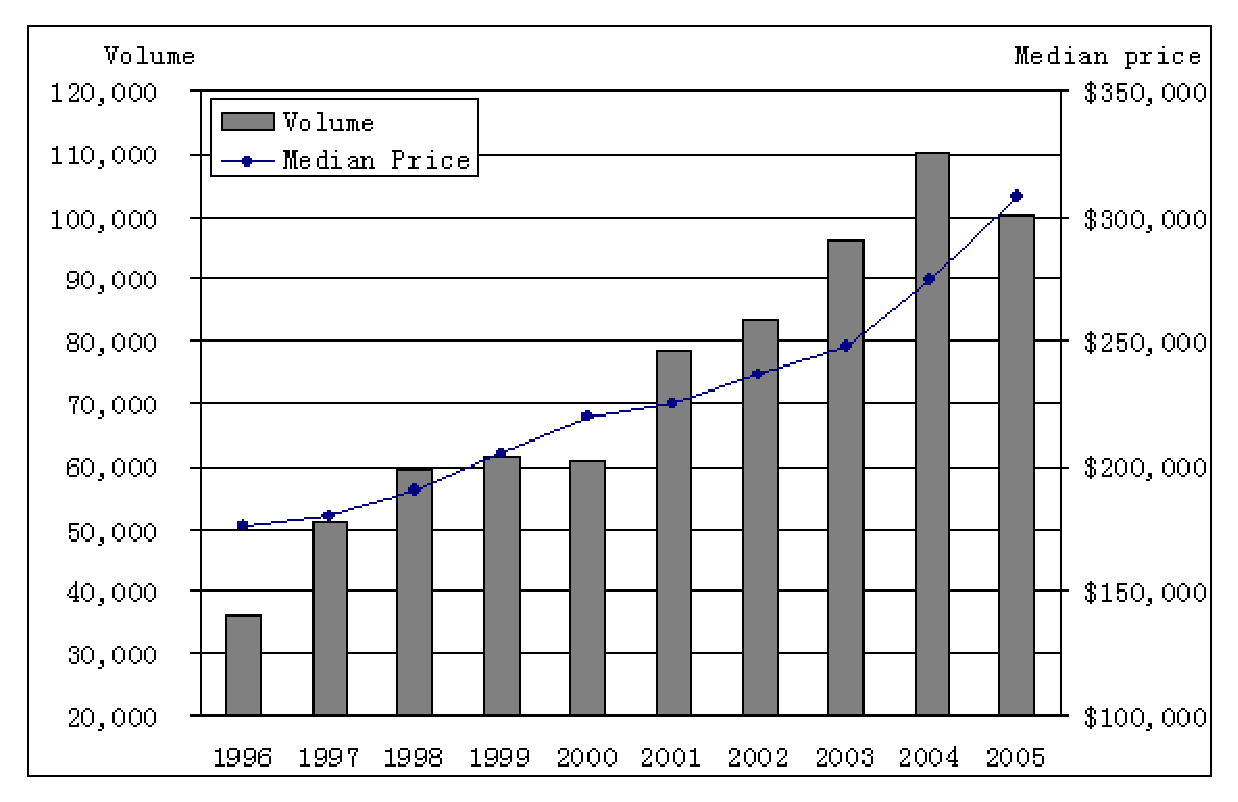
\includegraphics[scale=.8]{pv.eps}
\caption{Median home price and trading volume}
\label{fig-price-vol}
\end{figure}

\subsection{Household Types}
Although Chattopadhyay~\citeyear{Chattopadhyay1998} has
tested that the effect of various categorizations based on
household characteristics on the overall benefit estimates
are negligible, we devise a categarization of households by
income and life cyle.  Table~\ref{table-category} shows the
categorization definition and number of observations in each
type. Note that distribution of household types isn't
consistent in survey as in all region households.  In this
case, corrections for group size are necessary to reflect
the fact that, all else equal, large groups have greater
probability than small groups of bidding successfully for a
particular site, which can be done after the estimation by
subtracting the alternative specific constant by $\ln \mid
N_t \mid,\, t \in T$, where $N_t$ denotes the number of
members of group $t$.

\begin{table}[p]
\begin{center}
\caption{Definition of household types and number of observations} \label{table-category}
% Table generated by Excel2LaTeX from sheet 'Sheet1'
\begin{tabular}{lrrrr}

\multicolumn{ 1}{c}{Category} & \multicolumn{ 1}{c}{Description} & \multicolumn{ 2}{c}{Observations} &            \\

\multicolumn{ 1}{c}{} & \multicolumn{ 1}{c}{} &  in region & \multicolumn{ 2}{|c}{in survey} \\
\hline
                      \multicolumn{ 1}{l}{Income} &            \\
\hline
       Low & 1/4 Quintile &    320,956 & \multicolumn{ 2}{l}{50} \\
\hline
    Median & 2/4-3/4 Quintile &    639,115 & \multicolumn{ 2}{l}{371} \\
\hline
      High & 4/4 Quintile &    325,837 & \multicolumn{ 2}{l}{100} \\
\hline
                  \multicolumn{ 1}{l}{Life Cycle} &            \\
\hline
Single or Young & \multicolumn{ 1}{l}{householder $<=$34, 1 or } & \multicolumn{ 1}{l}{325,837} & \multicolumn{ 2}{l}{63} \\

    Couple & \multicolumn{ 1}{l}{2 persons, w/o children} & \multicolumn{ 1}{l}{} &   \multicolumn{ 2}{l}{} \\
\hline
Household with school age children & $>=$2 persons, w/ children &    428,272 & \multicolumn{ 2}{l}{240} \\
\hline
Empty Nester & householder 35-64, w/o children &    455,316 & \multicolumn{ 2}{l}{164} \\
\hline
Senior household & householder $>=$ 64, w/o children &    208,344 &         49 &            \\

\end{tabular}  


\end{center}
\end{table}
%\begin{figure}[htb]
%\centering
%\includegraphics{category1.eps}
%\caption{Table Definition of household types and number of observations}
%\label{table-category}
%\end{figure}

\section{Estimation Results}
\label{results}

\subsection{Household Location Choice Model}

Estimation results of Household Location Choice Model is shown in Table~\ref{table-hlcm}.

\begin{table}[p]
\begin{center}
\caption{Estimation Results of Household Locatin Choice Model} \label{table-hlcm}
% Table generated by Excel2LaTeX from sheet 'hlcm'
\begin{tabular}{p{2in}rrrr}

variable name & coefficient name &   estimate & standard error & t statistic \\
\hline
housing cost to income ratio &        RCI & -0.585449994 &   0.058869 & -9.944996834 \\

percent residential land within walking distance &        PRW & 0.018315436 &   0.001229 & 14.90827084 \\

income interacts log of  improvement value per unit &     IIMPPU &   8.11E-06 &   6.53E-07 & 12.42929268 \\

log of residential units &        LDU & 0.079023123 &   0.027113 & 2.914613724 \\

ln retail sector employment within walking distance if household has less cars than workers &      LRWCW & 0.280604362 &   0.030556 & 9.183265686 \\

percent high income households within walking distance if household is high income &      HIHIW & 0.017414367 &   0.003696 & 4.712301254 \\

percent low income households within walking distance if household is low income &      LILIW & 0.018685734 &   0.003655 & 5.111677647 \\

percent mid income households within walking distance if household is mid income &      MIMIW & 0.019969231 &   0.003615 & 5.524710655 \\

percent minority households within walking distance if household is minority &       MPMW & 0.019145619 &   0.004975 & 3.848261356 \\

percent minority households within walking distance if household is not minority&      NMPMW & -0.019966682 &   0.002445 & -8.164773941 \\

residential units when household has children &        UCH & -0.016478887 &   0.001337 & -12.3238287 \\

log of travel time weighted access to employment &     GWAEDA & 0.296539605 &   0.036159 & 8.200985909 \\
\hline
\end{tabular}  


\end{center}
\end{table}

\subsection{Random Bidding Model}
Estimation results for categorization of income groups (low, mid and high income) are presented in Table~\ref{table-rbm1}, with 520 observation and $\rho^2 = 0.23$ %Table~\ref{tab-rbm2} for income and life cycle categorization respectively.

\begin{table}[p]
\begin{center}
\caption{Estimation Results of Random Bidding Model} \label{table-rbm1}
% Table generated by Excel2LaTeX from sheet 'Sheet3'
\begin{tabular}{p{2in}rrrrrrr}

           &      \multicolumn{ 3}{c}{Low Income} &            &     \multicolumn{ 3}{c}{High Income} \\

           &      Coef. &  Std. Err. &        P$>$z &            &      Coef. &  Std. Err. &        P$>$z \\
\hline
  bedrooms &   0.277896 &    0.14359 &      0.053 &            &   0.230516 &   0.120369 &      0.055 \\

 bathrooms &   -0.50053 &   0.237347 &      0.035 &            &          - &            &            \\

dummy for high quality building &          - &            &            &            &   0.647945 &   0.360053 &      0.072 \\

dummy for low quality building &   0.802767 &    0.29401 &      0.006 &            &          - &            &            \\

travel time to CBD &          - &            &            &            &   0.014613 &   0.005409 &      0.007 \\

improvement values (in thousands) &   -0.01532 &   0.002621 &          0 &            &          - &            &            \\

percent high income within walking distance &          - &            &            &            &   0.093292 &   0.010295 &          0 \\

number of jobs within 30 mins of transit \& walk &   3.62E-05 &   1.66E-05 &      0.029 &            &   3.63E-05 &   1.77E-05 &       0.04 \\

building sqft &   0.000355 &   8.87E-05 &          0 &            &    -0.0006 &    0.00011 &          0 \\

alt. specific constant &   -0.43466 &   0.431302 &      0.314 &            &   -4.25146 &   0.616193 &          0 \\
\hline
\end{tabular}  


\end{center}
\end{table}

Estimation results for categorization of life cycle groups (Single and Young Couple, Household with Children, Empty Nester, and Senior Household) are presented in Table~\ref{table-rbm2}, with 517 observation and $\rho^2 = 0.08$
\begin{table}[p]
\begin{center}
\caption{Estimation Results of Random Bidding Model} \label{table-rbm2}
% Table generated by Excel2LaTeX from sheet 'Sheet1'
\begin{tabular}{p{1in}rrrrrrrrrrr}

           & \multicolumn{ 3}{c}{Single \& Young Couple} &            &    \multicolumn{ 3}{c}{Empty Nester} &            &          \multicolumn{ 3}{c}{Senior} \\
\hline
           &      Coef. &  Std. Err. &        P$>$z &            &      Coef. &  Std. Err. &        P$>$z &            &      Coef. &  Std. Err. &        P$>$z \\
\hline
  bedrooms &          - &            &            &            &   -0.29974 &   0.093314 &      0.001 &            &          - &            &            \\

dummy for low quality building &          - &            &            &            &   -0.54917 &   0.276618 &      0.047 &            &    -0.8587 &   0.473263 &       0.07 \\

improvement values (in thousands) &   -0.00516 &   0.001646 &      0.002 &            &          - &            &            &            &   -0.00294 &     0.0005 &          0 \\

building sqft &          - &            &            &            &   -0.00024 &   5.51E-05 &          0 &            &          - &            &            \\

housing density &    0.30502 &   0.059121 &          0 &            &          - &            &            &            &          - &            &            \\

alt. specific constant &   -1.89085 &   0.318252 &          0 &            &    0.82217 &   0.326036 &      0.012 &            &   -1.28623 &    0.18525 &          0 \\

           &            &            &            &            &            &            &            &            &            &            &            \\
\hline
\end{tabular}  


\end{center}
\end{table}

\section{Discussion and Further Development}
\label{future-work}

The two models presented in this paper capture complementary aspects of the housing market:
the consumer choice of housing, and the seller choice among bidders and the transaction price.  We propose
to integrate these two perspectives in a unified model.  Some work along this line has been developed by
Martines and Hurtuba (2006), in which they model the probability that a household of type \emph{h} is the winning bidder for a property, as a function of the bids of these households, and
the number of households of each type $\overline{H}$:

\begin{equation}
\label{eq_p_t2}
p(t \mid z)=\frac{\overline{H} exp(\tilde{\psi}_t(z))}{\sum_{t^\prime \in T}{\overline{H} exp(\tilde{\psi}_t^\prime(z))}}.
\end{equation}

The number of households of each type $\overline{H}$ is equivalent to a size adjustment in the standard Ellickson
random bidding model, shown in equation \ref{eq_p_t2}.  In their formulation of a bid function, Martinez and Hurtuba include
the household composition of each location, thereby making the bid of each household that is on the right hand side a
function of $\overline{H}$, which is itself an outcome of the result of the competitive bidding process.  In other words, the
model is not directly solvable due to this simultaneity.  Their approach to the simultaneity is to formulate it as a fixed point problem
and find a computational solution to a system of equations that is based on an assumption of joint maximization of the utilities
of all buyers and sellers in the market at equilibrium.  They have formulated a mathematical solution for this, but
have not reported standard econometric results such as parameter estimates or standard errors, or other
measures of goodness of fit.

In our proposed approach, now in development, we take a more econometric approach
to the integration of Ellickson's random bidding model and the household location choice model.  We treat the simultaneity problem
outlined above as an econometric endogeneity, and propose an iterative estimation strategy to couple these models.  We propose the
following algorithm for estimating consistent parameters for a model system comprised of these location choice and random bidding
equations, stratified by household type and housing type:

\begin{itemize}

\item Estimate the household location choice model using standard MNL techniques as applied in this paper, using observed prices and $\overline{H}$
in the utility specification to reflect preferences for social composition of the neighborhood.
\item Use the estimated parameters to predict individual location choice probabilities.
\item Sum the probabilities across households for each property or location, to obtain initial estimates of $\overline{H}_{h}$ for each.
\item Use the estimated $\overline{H}_{h}$ in the estimation of the parameters of a random bidding model.
\item Use the estimated parameters of the random bidding model to predict prices and the distrbition of winning bidders $\overline{H}$.
\item Repeat the process beginning with step 1, replacing the observed prices and $\overline{H}$ with those generated from the random bidding model.
\item Terminate iteration of the estimation of the location choice model and the random bidding model when the $\overline{H}$ and price vectors have
converged to a stable state, within a user-specified tolerance.

\end{itemize}

The convergence properties of the proposed algorithm have not yet been developed, nor has the algorithm been implemented at this time.
Once these aspects are completed, we intend to apply the model to a policy analysis of the dynamics of the housing market in the Puget Sound
region, to explore patterns of gentrification and the potential efficacy of alternative interventions via demand side, supply side regulatory
 and pricing strategies, in addition to transportation policies.


\bibliographystyle{agsm}
\bibliography{workon}

\end{document}


